\documentclass{llncs}
\usepackage{amsmath,amssymb,graphicx,multirow,listings,hyperref}
\usepackage{epstopdf}


%\makeatletter
%\newcommand{\sboxed}[1]{\setlength{\fboxsep}{0.7pt}\fbox{\m@th$\displaystyle#1$}}
%\makeatother

\newcommand{\sboxed}[1]{\textbf{#1}}


\newcommand{\thet}[1]{\theta_{\sboxed{#1}}}
\newcommand{\ft}{\left(f,t\right)}
\newcommand{\ftt}[1]{\left(f,t\mid\thet{#1}\right)}




\begin{document}
\title{The 2018 Signal Separation Evaluation Campaign}
\author{
Antoine Liutkus\inst{1} \and
Fabian-Robert St\"{o}ter\inst{1} \and
Nobutaka Ito\inst{2}
}

\institute{
Inria and LIRMM, University of Montpellier, France\and
NTT Communication Science Laboratories, NTT Corporation, Japan
}

\maketitle
%
\vspace{-3mm}
\begin{abstract}
This paper reports the organization and results for the 2018 community-based Signal Separation Evaluation Campaign (SiSEC 2018). This year's edition was focused on audio and pursued the effort towards scaling up and making it easier to prototype audio separation software in an era of machine-learning based systems. For this purpose, open-source software was developed and released to automatically load, process and report performance on the new MUSDB'18 music separation database. Additionally, a new official Python~3 version for the \texttt{BSS~Eval} toolbox was released, along with reference implementations for three oracle separation methods: ideal binary mask, ideal ratio mask, and multichannel Wiener filter.
\end{abstract}

\setcounter{footnote}{0}
\section{Introduction}
\vspace{-2mm}
Source separation is a signal processing problem that consists in recovering individual superimposed \textit{sources} from a \textit{mixture}.  Since 2008, the role of the Signal Separation Evaluation Campaign (SiSEC) has been to compare performance of separation systems on a volontary and community-based basis, by defining tasks, datasets and metrics to evaluate methods~\cite{sassec2007,sisec2008,sisec0710,sisec2011,sisec2013,sisec2015,sisec2016}. Although source separation may find applications in several domains, the focus of SiSEC has always mostly been on audio source separation, with tasks pertaining to both speech and music separation.

This year, we decided to drop the legacy speech separation and denoising tasks UND and BGN, because they are now the core focus of very large and successful other campaigns such as CHiME~\cite{chime,chime2,chime3}. Instead, most of our efforts were spent on music separation, where the SiSEC MUS task is playing an important role, both in terms of datasets and participation.


%\begin{figure*}[t]
%  \begin{center}
%     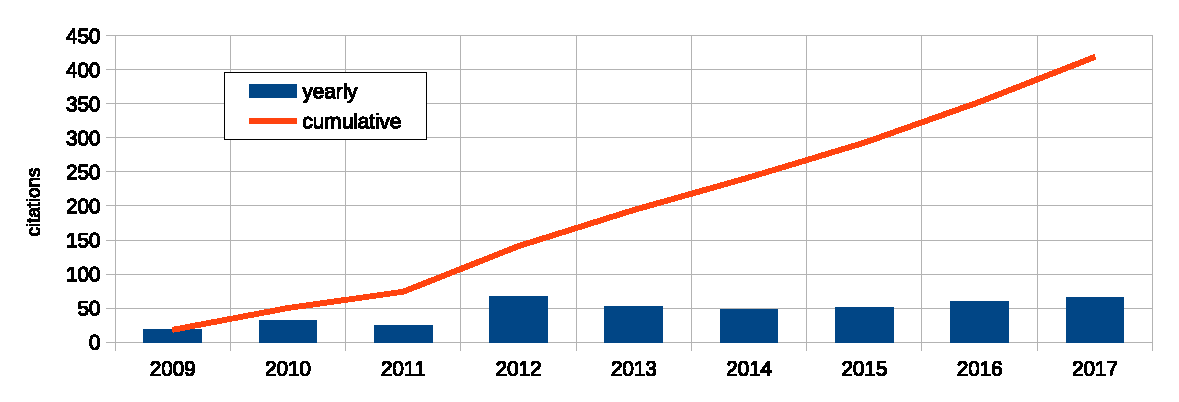
\includegraphics[width=\linewidth]{fig/SiSEC_impact.eps}
%     \vspace{-1cm}
%  \end{center}
%  \caption{The number of papers referring to SiSEC (source: Google Scholar).}
%  \label{fig:SiSEC_pub}
%\end{figure*}

While the primary objective of SiSEC is to regularly report on the progress made by the community through standardized evaluations, its secondary objective is also to provide useful resources for research in source separation, even outside the scope of the campaign itself. This explains why the SiSEC data has always been made public, so that it could be used for related publications. %Over the years, it has a moderate, but significant impact on the audio research, as seen on Figure~\ref{fig:SiSEC_pub}.

Since 2015, the scope of the SiSEC MUS data was significantly widened, so that it could serve not only for evaluation, but also for the design of separation system. This important shift in the purpose of the SiSEC data is motivated by the important development of systems based on deep learning, which now define the state-of-the-art and require important amounts of learning data. This lead to the proposal of the MSD~\cite{sisec2015} and the DSD100~\cite{sisec2016} datasets, that were used in the previous two SiSEC.

This year's SiSEC present several contributions. First, the computation of oracle performance goes further than the usual Ideal Binary Mask (IBM) method to also include Ideal Ratio Mask (IRM) and Multichannel Wiener Filters (MWF). Second, we continued our effort in gathering a dataset for training music separation systems and released the MUSDB'18, that comprises almost 10~h of music with separated stems. Third, we released a new version~4 for the \texttt{BSS~Eval} toolbox, that handles time-invariant distortion filters, significantly speeding up computations. Fourth, we provide the community with plotting tools to be used for quickly reporting the performance of new systems. Pointers to open-source implementations in Python~3 for all these contributions may be found in the SiSEC website\footnote{\url{sisec.inria.fr}.}.

\section{Oracle performance for audio separation}
We write $I$ as he number of channels of the audio mixture: $I=2$ for stereo. We write $x$ for the 3-dimensional complex array obtained by stacking the Short-Time Frequency Transforms (STFT) of all channels. Its dimensions are $F\times T\times I$, where $F,T$ stand for the number of frequency bands and time frames, respectively. Its values at Time-Frequency (TF) bin $\ft$ are  written $x\ft\in\mathbb{C}^I$, with entries $x_i\ft$. The mixture is taken as the sum of the sources \textit{images}: $x\ft=\sum_j y_j\ft$, which correspond to the isolated instruments and are also multichannel.

A filtering method $\sboxed{m}$ usually computes estimates $\hat{y}_j^{\sboxed{m}}$ for the source images linearly from $x$:
\begin{equation}
  \hat{y}_j^{\sboxed{m}}\ftt{m}=M_j^{\sboxed{m}}\ftt{m} x\ft,\label{eq:TFmask}
\end{equation}
where $\thet{m}$ are some parameters specific to $\sboxed{m}$ and $M_j\ftt{m}$ is a $I\times I$ complex matrix called a TF \textit{mask}, computed using $\thet{m}$ in a way specific to method~$\sboxed{m}$. Once given the filtering strategy $\sboxed{m}$, the objective of a source separation system is to analyze the mixture to obtain parameters $\thet{m}$ that yield good separation performance.

For evaluation purposes, it is useful to know how good a filtering strategy can get, i.e. to have some upper bound on its performance, which is what an \textit{oracle} is~\cite{vincent2007oracle}:
\begin{equation}
  \thet{m}^{\star}=\underset{\thet{m}}{\text{argmin}}\sum_{f,t}\left\Vert y_{j}\ft-\hat{y}_{j}^{\sboxed{m}}\ftt{m}\right\Vert,
  \end{equation}
where $\Vert\cdot\Vert$ is any norm deemed appropriate. In this SiSEC, we covered the three most commonly used filtering strategies, and assessed performance of their respective oracles:
\begin{enumerate}
  \item The \textbf{Ideal Binary Mask} (IBM,~\cite{wang2005}) is arguably the simplest filtering method. It processes all $\left(f,t,i\right)$ of the mixture independently and simply assigns each of them to one source only:   $M_{ij}^\sboxed{IBM}\ft\in\left\{0,1\right\}$. Its oracle performance is obtained if the source with strongest magnitude is picked each time.
  \item The \textbf{Ideal Ratio Mask} (IRM), also called the $\alpha$-Wiener filter~\cite{liutkus15}, relaxes the binary nature of the IBM. It processes all $\left(f,t,i\right)$ through multiplication by $M_{ij}^\sboxed{irm}\in\left[0,1\right]$ defined as:
  \begin{equation}
    M^{\sboxed{IRM}}_{ij}\ft=\frac{v_{ij}\ft}{\sum_{j'}v_{ij'}\ft},
  \end{equation}
where $v_{ij}\ft=\left|y_{ij}\ft\right|^\alpha$ is the fractional power spectrogram of the source image $y_{ij}$. Particular cases include the Wiener filter for $\alpha=2$.
  \item The \textbf{Multichannel Wiener Filter} (MWF, \cite{duong10}) exploits multichannel information, while IBM and IRM do not. $M^{\sboxed{MWF}}_{j}\ft$ is a $I\times I$ complex matrix given by:
  \begin{equation}
    M_{j}^{\sboxed{MWF}}\ft=C_{j}\ft C_{x}\ft,
  \end{equation}
where $C_j\ft$ is the $I\times I$ covariance matrix for source $j$ at TF bin $\ft$ and $C_x=\sum_j C_j$. In the classical local Gaussian model \cite{duong10}, the further parameterization $C_j\ft=v_j\ft R_j\left(f\right)$ is picked, with $R_j$ being the $I\times I$ \textit{spatial covariance matrix}, encoding the average correlations between channels at frequency bin $f$, and $v_j\ft\geq0$ encoding the power spectral density at $\ft$. The optimal values for these parameters are easily computed from the true sources $y_j$ \cite{liutkus2013}.
\end{enumerate}

These three oracle systems have been implemented in Python~3 and released in an open-source license\footnote{\url{github.com/sigsep/sigsep-mus-oracle}}.

\section{Data and metrics}

\subsection{The MUSDB18 Dataset}
For the organization of the present SiSEC, the MUSDB18 corpus was released~\cite{musdb18}, that comprises tracks from MedleyDB~\cite{medleydb}, DSD100~\cite{sisec2015,sisec2016}, and other material. In total, it features $150$ full-length tracks for approximately~$10$~h of audio. Its noticeable features are the following.
\begin{itemize}
\item All items are full-length tracks, so that the handling of long-term musical structures, and of silent regions in the lead/vocal signal, can be evaluated.
\item It only features stereo signals which were mixed using professional digital audio workstations. This results in quality stereo mixes which are representative of real application scenarios.
\item As for the previous SiSEC official dataset DSD100, all signals are split into 4 predefined categories: bass, drums, vocals, and other. This contrasts with the finer granularity of MedleyDB, but promotes automation of the algorithms.
\item Many musical genres are represented in MUSDB, for example, jazz, electro, metal, etc.
\item It is split into a development (100 tracks, 6.5~h) and a test dataset (50 tracks, 3.5~h), for the design of data-driven separation methods.
\end{itemize}
The dataset is freely available for download online, along with Python~3 development tools\footnote{\url{https://sigsep.github.io/musdb}}.

\subsection{BSS Eval version~4}
The BSS~Eval metrics, as implemented in the MATLAB toolboxes~\cite{bssevalv2,bssevalv3} are widely used in the audio separation literature. They quantify the discrepancies between true sources and their estimates through $3$~criteria: Source to Distortion, to Artefact, to Interference ratios (SDR, SAR, SIR) and additionally with the Image to Spatial distortion (ISR) for the \texttt{BSS~Eval v3} toolbox~\cite{bssevalv3}.

One particularity of BSS~Eval is to compute the metrics after optimally matching the estimates to the true sources through linear \textit{distortion filters}. This arguably allows the criteria to be robust to some linear mismatches. Apart from the optional computation of all possible permutations of the sources, this matching is the reason for most of the computation cost of BSS~Eval, especially considering it is done for each evaluation window when the metrics are computed on a framewise basis.

In this SiSEC, we decided to drop the assumption that distortion filters could be varying over time, but considered instead they are fixed for the whole length of the track. First, this significantly reduces the computational cost for evaluation because matching needs to be done only once for the whole signal. Second, this introduces much more dynamics in the evaluation, because time-varying matching filters turn out to over-estimate performance, as we show in Section~\ref{ssec:bsseval-results}. Third, this makes matching more robust, because true sources are not silent throughout the whole recording, while they often were for short windows.\footnote{We also only use the BSSeval \texttt{images} version, as defined in~\cite{bssevalv3}, because the \texttt{sources} version~\cite{bssevalv2} suffers from strong instabilities in some borderline cases such as silent estimates.}

This new $4^{th}$ version for the \texttt{BSS~Eval} toolbox was implemented in Python~3, and allows either time-invariant or time-varying distortion filters. In the latter case, it is fully compatible with earlier MATLAB-based versions up to a tolerance of $10^-7$~dB. It may be found through classical Python~3 package manager or on the dedicated website\footnote{\texttt{pip3 install bsseval} or \url{bass-db.gforge.inria.fr/bss_eval/}}.

\section{Separation results}
\subsection{Oracle performance with \texttt{BSS Eval v4}}
\label{ssec:bsseval-results}
\subsection{Comparison of systems submitted to SiSEC-MUS 2018}
\subsection{Comparison of systems submitted to SiSEC-ASY 2018}
To be completed when the results have been submitted, for the camera-ready version.

\section{Conclusion}
\label{sec:concl}
\vspace{-2mm}
We reported our work on the organization of SiSEC 2018, that comprised the development of a new Python version~$4$ for BSS~Eval to assess performance, which is fully compatible with earlier MATLAB versions and additionally allows for time-invariant distortion filters, significantly reducing computational load. Furthermore, we presented the new MUSDB'18 dataset, that gathers 150 music tracks with isolated stems, totaling almost $10$~h of music for the design and evaluation of music separation systems. Finally, we also provide open-source implementations of~$3$ popular oracle methods to assess upper bounds for performance.

Then, we reported the impact of choosing time-invariant distortion filters for the new BSS~Eval~v4 over time-varying ones as done before. The discussion was conducted based on the performance of the proposed implementations for oracle methods.

Finally, we provided an overall presentation of the scores obtained by the participants to this year's edition. More detailed analysis and sound excerpts to be listened to can be accessed online on the SiSEC webpage.
\footnotesize
\bibliographystyle{plain}
\bibliography{references}
\end{document}
